\begin{figure}[tbp]
  \centering
  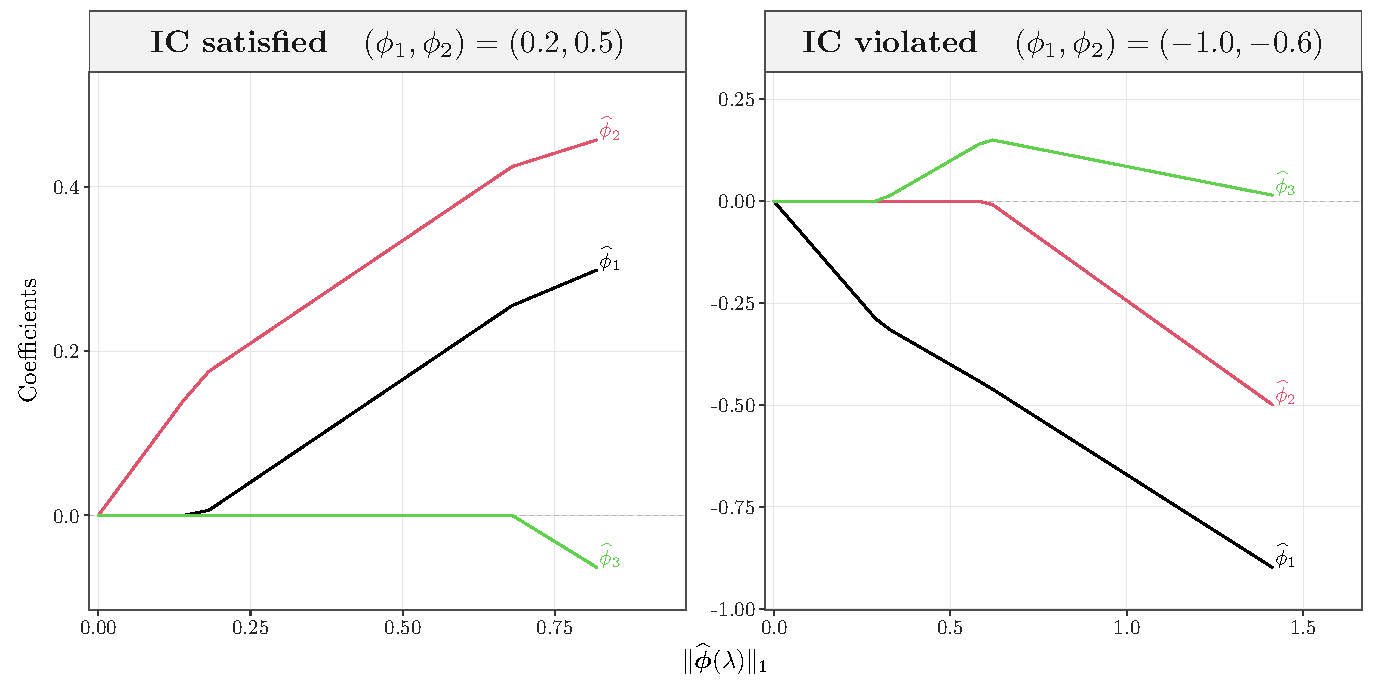
\includegraphics[width=\textwidth]{figures/fig01_04_ar_ir_condition_glmnet_v6.pdf}
  \caption{LASSO coefficient paths for an AR$(2)$ process fitted by an AR$(3)$ model. 
  Left: $(\phi_1,\phi_2)=(0.2,0.5)$, which satisfies both the causality condition (CC) 
  and the irrepresentability condition (IC). Right: $(\phi_1,\phi_2)=(-1,-0.6)$, 
  which is causal but violates IC. The horizontal axis is the $\ell_1$ norm along 
  the solution path, and the three curves correspond to the three fitted lag 
  coefficients. In both fits the true third-lag coefficient is zero. When IC holds 
  (left), $\widehat{\phi}_3$ remains close to zero along the path; when IC fails 
  (right), the inactive third-lag coefficient enters the LASSO path, illustrating 
  that causality alone does not guarantee exclusion of a spurious lag.}
  \label{fig:vars-ar2-lasso-paths}
\end{figure}
